\documentclass{beamer}
% This is the file main.tex
\usetheme{Dresden}
\usepackage{tikz}
\setbeamertemplate{navigation symbols}{}
\setbeamertemplate{mini frames}{}
\renewcommand*{\slideentry}[6]{}
\addtobeamertemplate{navigation symbols}{}{%
    \usebeamerfont{footline}%
    \usebeamercolor[fg]{footline}%
    \hspace{1em}%
    \insertframenumber/\inserttotalframenumber
}
\setbeamercolor{structure}{fg=MyPurple}
\definecolor{MyPurple}{RGB}{105,18,83}
\usepackage{graphicx}
\usepackage{amsmath}
\usepackage[euler]{textgreek}
\usepackage{adjustbox}
\usepackage{booktabs}
\usepackage{multirow}
\usepackage{multirow, xspace, amsmath}
\usepackage{pdfpages}
\usepackage{fancybox}
\usepackage{stackengine}
\usepackage{cancel}
%\usepackage{geometry}
%\geometry{
% a4paper,
% total={170mm,257mm},
% left=20mm,
% top=20mm,
% }
\newcommand*{\ttbar}{\ensuremath{t\bar{t}}\xspace}
\newcommand*{\mbb}{\ensuremath{\text{m}_{bb}}\xspace}
\newcommand*{\dsig}{\ensuremath{|\sigma_{d_{0}}|}\xspace} 
\newcommand*{\met}{\ensuremath{\cancel{E_{T}}}\xspace}
\newcommand{\backupbegin}{
   \newcounter{framenumberappendix}
   \setcounter{framenumberappendix}{\value{framenumber}}
}
\newcommand{\backupend}{
   \addtocounter{framenumberappendix}{-\value{framenumber}}
   \addtocounter{framenumber}{\value{framenumberappendix}} 
}
\newcommand\tab[1][1cm]{\hspace*{#1}}

\newcommand*{\header}[1]{\fontsize{16}{8}\selectfont \textbf{{\color{MyPurple}{#1}}}}

\usepackage{tikz}
\usepackage[compat=1.1.0]{tikz-feynman}


\title{Search For Double Higgs Production in the $b\bar{b}WW^{*}$ Channel}
\subtitle{}
\author[John C.S. Myers]{John C.S. Myers}
\institute[University of Oregon]{ University of Oregon}
\date{\today}

\begin{document}

\titlepage
%%Start with general into and then briefly on trigger
%% highlight talks and being public face
%%
%%need to think of transiton into HHbbWW
%%
%%HHbbWW paper analysis-->leptons inside jets-->how to use ANL computing


\begin{frame}
\begin{center}
\header{Overview}
\end{center}
\begin{itemize}
%\small
\item The Standard Model
\begin{itemize}
%\footnotesize
\item Higgs Physics
\end{itemize}
\item BSM Di-Higgs Production
\item The LHC and ATLAS
\item $HH\rightarrow{}b\bar{b}WW^{*}$ Analysis
\item Improvements to the Analysis
\item Conclusion and Outlook
\end{itemize}
\end{frame}

\begin{frame}
\begin{center}
\header{The Standard Model}
\end{center}
\begin{columns}
\begin{column}{0.5\textwidth}
\begin{itemize}
\item Describes matter (fermions) and force carriers (gauge bosons)
\item Very successful model
\item Final piece (Higgs Boson) discovered in 2012
\end{itemize}
\end{column}
\begin{column}{0.5\textwidth}
\includegraphics[width=1\textwidth]{figures/Standard_Model_of_Elementary_Particles}
\end{column}
\end{columns}
\end{frame}

\begin{frame}
\begin{center}
\header{Higgs Mechanism}
\end{center}
\begin{columns}
\begin{column}{0.5\textwidth}
\color{MyPurple}{Scalar Boson}\color{black}
\begin{center}
$\phi_0 = \frac{1}{\sqrt{2}}\binom{0}{v}$\\~\\
\huge$\Downarrow$ \normalsize EWSB \huge$\Downarrow$ \normalsize\\~\\
$\phi(x) = \frac{1}{\sqrt{2}}\binom{0}{v + h(x)}$\\~\\
Coupling to Gauge Bosons gives $W^{\pm},\ Z,\ A(\gamma)$\\~\\
$M_W^2 = \frac{1}{4}g^2v^2$\\~\\
\vspace{-0.3cm}$M_Z^2 = \frac{1}{4}(g^2 + g'^{2})v^2$\\~\\
\vspace{-0.3cm}$M_A^2 = 0$
\end{center}
\end{column}
\begin{column}{0.5\textwidth}
\includegraphics[width=1\textwidth]{figures/Higgs_mech}
\end{column}
\end{columns}
\end{frame}

\begin{frame}
\begin{center}
\header{Higgs Self-Coupling}
\end{center}
\begin{columns}
\begin{column}{0.5\textwidth}
\includegraphics[width=1\textwidth]{figures/higgspotential}
\end{column}
\begin{column}{0.5\textwidth}
\color{MyPurple}{Higgs Potential}\color{black}
\begin{center}
$V = \mu^2|\Phi^{\dagger}\Phi| + \lambda(|\Phi^{\dagger}\Phi|)^2$\\~\\
Expand self-coupling around VEV\\~\\
$V_\mathrm{self-coupling} \supset{} \lambda{}v\Phi^3 + \frac{\lambda}{4}\Phi^4$\\~\\
Tri-linear Higgs coupling strength $\lambda_{HHH}\equiv{}\lambda v$
\end{center}
\end{column}
\end{columns}
\end{frame}

\begin{frame}
\begin{center}
\header{Higgs Self-Coupling}
\end{center}
\begin{columns}
\begin{column}{0.5\textwidth}
\begin{center}
\includegraphics[width=0.75\textwidth]{figures/sm_fey}\\~\\
SM Theory cross section:\\
\small$\sigma_{\mathrm{HH}} \approx 33.53\mathrm{fb}$
\end{center}
\end{column}
\begin{column}{0.5\textwidth}
Two Dominant production modes at the LHC\\~\\
Interfere destructively to give small theoretical cross section\\
\begin{center}
\includegraphics[width=0.75\textwidth]{figures/SM_continuum}
\end{center}
\end{column}
\end{columns}
\end{frame}


\begin{frame}
\begin{center}
\header{Motivation}
\end{center}
\begin{columns}
\begin{column}{0.5\textwidth}
\textcolor{MyPurple}{Resonant di-Higgs production}\\
\begin{itemize}
\item A New process could decay to $HH$
\item E.g. Real Higgs Singlet Extension
\begin{itemize}
\item Couples to SM Higgs
\item Large enhancement to HH production rate
\begin{itemize}
\item Up to 30 times SM 
\end{itemize}
\end{itemize}
\end{itemize}
\end{column}
\begin{column}{0.5\textwidth}
\begin{figure}[h]
\footnotesize
\begin{center}
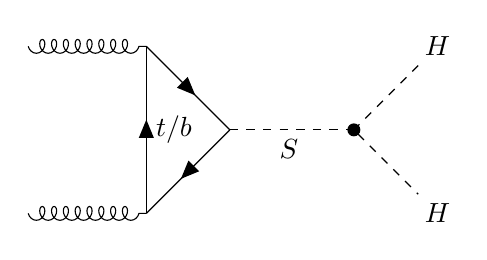
\begin{tikzpicture}
\begin{feynman}
\vertex (i1);
\vertex [right = of i1] (t1);
\vertex [dot][below right =of t1] (t3);
\vertex [below left= of t3] (t2);
\vertex [left = of t2] (i2);
\vertex [right =of t3][dot](h){};
\vertex [above right = of h] (f1){\(H\)};
\vertex [below right = of h] (f2){\(H\)};
\diagram* {
(i1) -- [gluon] (t1),
(i2) -- [gluon] (t2),
(t1) -- [fermion](t3) -- [fermion] (t2) -- [fermion,edge label'=\(t/b\)](t1),
(t3) -- [scalar,edge label'=\(S\)] (h),
(f1) -- [scalar] (h) -- [scalar](f2)
};
\end{feynman}
\end{tikzpicture}\\
\includegraphics[width=0.75\textwidth]{figures/ian6}
\end{center}
\end{figure}
\end{column}
\end{columns}
\end{frame}

\begin{frame}
\begin{center}
\header{The Large Hadron Collider}
\end{center}
\begin{center}
\includegraphics[width=1\textwidth]{figures/LHC}
\end{center}
\begin{columns}
\begin{column}{0.5\textwidth}
\begin{itemize}
\small
\item 13 TeV Proton-Proton Collider
\item 27 Km Circumference under the French-Swiss border
\end{itemize}
\end{column}
\begin{column}{0.5\textwidth}
\begin{itemize}
\small
\item 4 primary interaction points, each with a dedicated detector
\end{itemize}
\end{column}
\end{columns}
\end{frame}

\begin{frame}
\begin{center}
\header{The ATLAS Detector}
\end{center}
\begin{center}
\includegraphics[width=0.75\textwidth]{figures/ATLAS_det}
\end{center}
\begin{columns}
\begin{column}{0.5\textwidth}
\begin{itemize}
\item General purpose detector
\end{itemize}
\end{column}
\begin{column}{0.5\textwidth}
\begin{itemize}
\item 3.9 T Toroid
\end{itemize}
\end{column}
\end{columns}
\end{frame}

\begin{frame}
\begin{center}
\header{ATLAS Trigger}
\end{center}
\begin{columns}
\begin{column}{0.5\textwidth}
\begin{itemize}
\item LHC has 40 MHZ Collision Rate
\begin{itemize}
\item $\sim$64 TB/s 
\end{itemize}
\item 2 Level Trigger System
\begin{itemize}
\item Level-1 Trigger (L1)
\item High Level Trigger (HLT)
\end{itemize}
\item Reduces rate from 40MHz to $\sim$2 kHz ($\sim$3 GB/s)
\end{itemize}
\end{column}
\begin{column}{0.5\textwidth}
\includegraphics[width=1\textwidth]{figures/run2TDAQ}
\end{column}
\end{columns}
\end{frame}

\begin{frame}
\begin{center}
\header{Particles in the Detector}
\end{center}
\begin{center}
\includegraphics[width=0.75\textwidth]{figures/layers}
\end{center}
\end{frame}

\begin{frame}
\begin{center}
\header{$b\bar{b}WW^{*}$ semi-leptonic channel}
\end{center}
\vspace{-0.6cm}
\begin{columns}
\begin{column}{0.5\textwidth}
\begin{itemize}
\item $b\bar{b}WW^*$ has the second highest BR behind $b\bar{b}b\bar{b}$
\begin{itemize}
\footnotesize
\item One of the W bosons is off-shell
\end{itemize}
\item $bbl\nu$ final state 
\begin{itemize}
\footnotesize
\item Lepton helps against QCD
\item Neutrino makes reco. more challenging
\end{itemize}
\end{itemize}
\end{column}
\begin{column}{0.5\textwidth}
\begin{center}
\includegraphics[width=01.2\textwidth]{figures/DiHiggsBRs}
%\includegraphics[width=0.75\textwidth]{figures/comb_limit}
\end{center}
\end{column}
\end{columns}
\end{frame}

\begin{frame}
\begin{center}
\header{${\mathbf{bbl\boldsymbol{\nu{}}}}$ Final State}
\end{center}
\begin{columns}
\begin{column}{0.5\textwidth}
\begin{itemize}
\item electron or muon
\item 2 b quarks
\item 2 light flavor quarks
\item \met
\end{itemize}
\end{column}
\begin{column}{0.5\textwidth}
\begin{center}
\includegraphics[width=1\textwidth]{figures/res_prod}
\end{center}
\end{column}
\end{columns}
\end{frame}


\begin{frame}
\begin{center}
\header{Jets}
\end{center}
\begin{itemize}
\item Quarks hadronize before they interact with the detector
\item Gives sprays of energy deposits
\item Energy deposits grouped together into ``Jets" by algorithms
\end{itemize}
\begin{center}
\includegraphics[height=0.5\textheight]{figures/antikt}
\end{center}
\end{frame}

\begin{frame}
\begin{center}
\header{Neutrinos}
\end{center}
\begin{itemize}
\item Neutrinos do not interact with detector
\item Have transverse (perpendicular to beam line) information from \met
\item Need another piece to fully reconstruct 4-momentum
\begin{itemize}
\item This analysis used Higgs mass
\end{itemize}
\end{itemize}
\begin{center}
\includegraphics[height=0.5\textheight]{figures/met}
\end{center}
\end{frame}

\begin{frame}
\begin{center}
\header{Background}
\begin{columns}
\begin{column}{0.3\textwidth}
\color{MyPurple}{Major}
\begin{itemize}
\small
\item \ttbar
\item W+Jets
\item QCD multijet
\end{itemize}
Minor
\begin{itemize}
\small
\item Z+Jets
\item Single Top
\item Diboson
\end{itemize}
\end{column}
\begin{column}{0.7\textwidth}
\begin{center}
\color{MyPurple}{\ttbar vs signal}
\end{center}
\begin{center}
\includegraphics[width=0.45\textwidth]{figures/cartoon_tt}
\includegraphics[width=0.45\textwidth]{figures/cartoon_hh_crop}
\end{center}
\end{column}
\end{columns}
\end{center}
\end{frame}

\begin{frame}
\begin{center}
\header{Resolved Event Selection}
\end{center}
\begin{center}
\includegraphics[width=1\textwidth]{figures/resolvedv2}
\end{center}
\end{frame}

\begin{frame}
\begin{center}
\header{Boosted Event Selection}
\end{center}
\begin{center}
\includegraphics[width=1\textwidth]{figures/boostedv2}
\end{center}
\end{frame}

\begin{frame}
\begin{center}
\header{Signal Region}
\end{center}
\begin{columns}
\begin{column}{0.5\textwidth}
\begin{center}
\color{MyPurple}{Resolved}
\begin{itemize}
\item \met
\item $p_T^{bb}$
\item $p_T^{WW}$
\item $m_{bb}\sim{}m_H$
\item $m_{HH}\sim{}m_{S}$
\end{itemize}
\end{center}
\end{column}
\begin{column}{0.5\textwidth}
\begin{center}
\vspace{-1.4cm}\color{MyPurple}{Boosted}
\end{center}
\begin{itemize}
\item \met
\item $m_\mathrm{Large-R\ jet}\sim{}m_H$
\end{itemize}
\end{column}
\end{columns}
\end{frame}

\begin{frame}
\begin{center}
\header{Resolved Background Determination}
\end{center}
\begin{columns}
\begin{column}{0.5\textwidth}
\color{MyPurple}{\ttbar}
\begin{itemize}
\footnotesize
\item Normalized in $m_{bb}$ CR
\begin{itemize}
\scriptsize
\item Boosted \ttbar VR
\end{itemize}
\end{itemize}
\end{column}
\begin{column}{0.5\textwidth}
\color{MyPurple}{Other MC Bkg.}
\begin{itemize}
\footnotesize
\item Modeled using MC and normilized to SM XSec
\end{itemize}
\end{column}
\end{columns}
\begin{center}
\color{MyPurple}{QCD multi-jet background}
\end{center}
\begin{columns}
\begin{column}{0.5\textwidth}
\begin{itemize}
\vspace{-0.5cm}
\footnotesize
\item ABCD data driven estimate
\begin{itemize}
\item $N_A = F N_C N_B / N_D$
\item $F$ is a correction factor determined earlier in the cutflow
\item Boosted uses $\met>50\text{ GeV}$
\begin{itemize}
\scriptsize
\item Takes shape from 1 b-tag C Region
\end{itemize}
\end{itemize}
\end{itemize}
\end{column}
\begin{column}{0.5\textwidth}
\includegraphics[width=0.9\textwidth]{figures/abcdExample_met_vs_d0sigBL20}
\end{column}
\end{columns}
\end{frame}

\begin{frame}
\begin{center}
\header{Background Shape Check}
\end{center}
\begin{center}
\includegraphics[width=0.8\textwidth]{figures/C_mBBcr_reOpt700_mww_bbpt210_wlepmtben_regionA_met25d020-eps-converted-to}
\end{center}
\small
$m_T = \sqrt{2p_T^l\met\times{}(1-\cos{\Delta{\phi}})}$
\end{frame}

\begin{frame}
\begin{center}
\header{Results}
\end{center}
\begin{center}
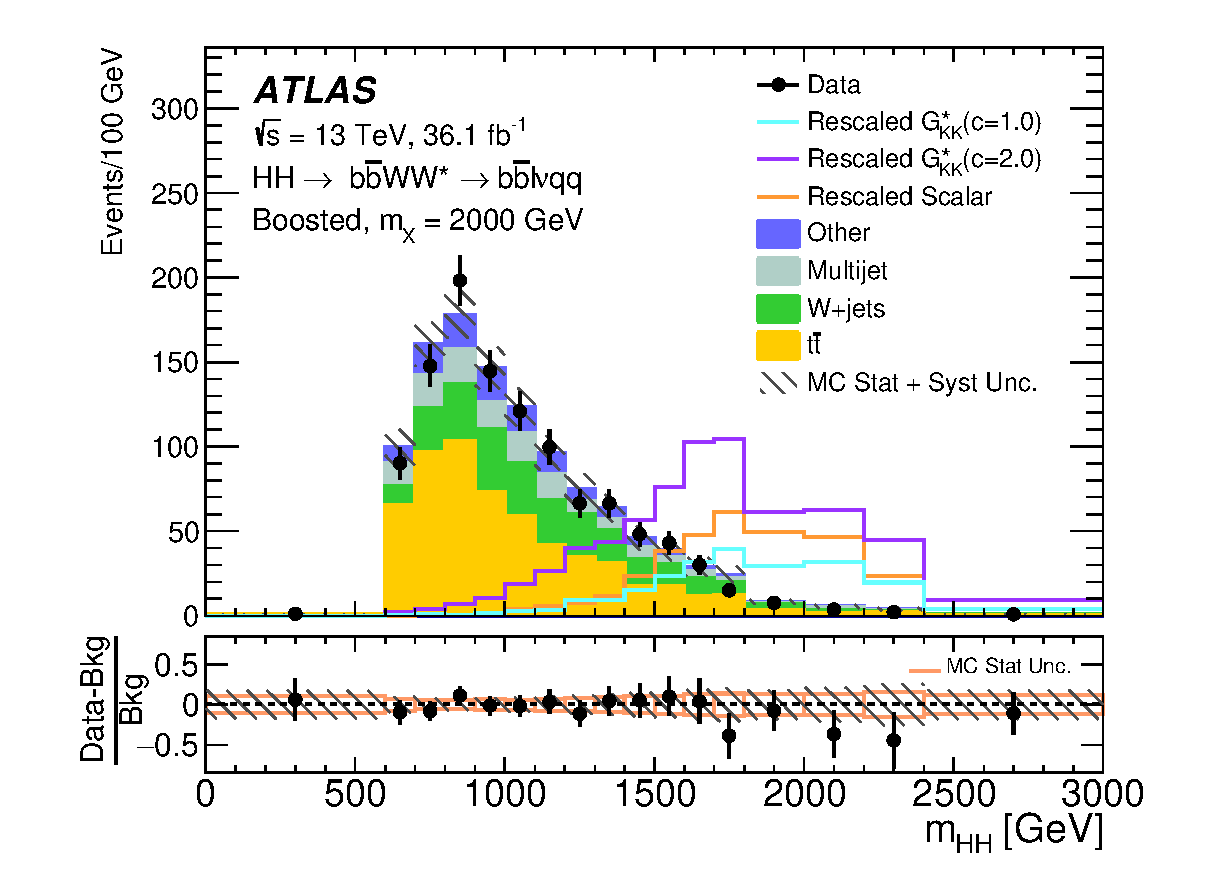
\includegraphics[width=0.8\textwidth]{figures/C_2tab_0bjet_SR_lepton_presel_met50_hhMassRebin1_postfit}
\end{center}
%\end{column}
%\end{columns}
\end{frame}

\begin{frame}
\begin{center}
\header{Combined Limit}
\end{center}
\begin{center}
\includegraphics[width=0.65\textwidth]{figures/limit_2016_reOpt_HiggsApproved_Scalar_Paper_Combined_20190312_01}
\end{center}
\small
\vspace{-0.5cm}$\sigma(pp\rightarrow{}HH)B(HH\rightarrow{}b\bar{b}WW^*) < 300^{+100}_{-80} \times{} SM$
\end{frame}

\begin{frame}
\begin{center}
\header{Motivation}
\end{center}
\vspace{-0.5cm}
\begin{columns}
\begin{column}{0.5\textwidth}
\begin{itemize}
\footnotesize
\item $H\rightarrow{}WW$ becomes boosted around 1 TeV 
\item Quarks become too close together to use 0.4 jets
\item Overlap removal with leptons kill efficiency
\item A "Fully-Boosted" selection recovers lost efficiency at high $m_S$
\end{itemize}
\end{column}
\begin{column}{0.5\textwidth}
\begin{center}
\includegraphics[width=0.75\textwidth]{figures/drminlq}
\end{center}
\end{column}
\end{columns}
\end{frame}

\begin{frame}
\begin{center}
\header{Fully Boosted Event Selection}
\end{center}
\begin{center}
\includegraphics[width=1\textwidth]{figures/fullboost}
\end{center}
\end{frame}

\begin{frame}
\begin{center}
\header{Signal Reconstruction}
\end{center}
\begin{columns}
\begin{column}{0.5\textwidth}
\includegraphics[width=01\textwidth]{figures/electron/mww_e}
\end{column}
\begin{column}{0.5\textwidth}
\includegraphics[width=01\textwidth]{figures/electron/mhh_e}
\end{column}
\end{columns}
\end{frame}

\begin{frame}
\begin{center}
\header{Background Modeling}
\end{center}
\begin{columns}
\begin{column}{0.5\textwidth}
\begin{itemize}
\item Same procedure as boosted paper analysis
\item Slightly looser selection to increase statistics
\item Check shape in mBB control region
\end{itemize}
\end{column}
\begin{column}{0.5\textwidth}
\includegraphics[width=1\textwidth]{figures/ABCD}
\end{column}
\end{columns}
\end{frame}

\begin{frame}
\begin{center}
\header{Background Shape Check}
\end{center}
\begin{center}
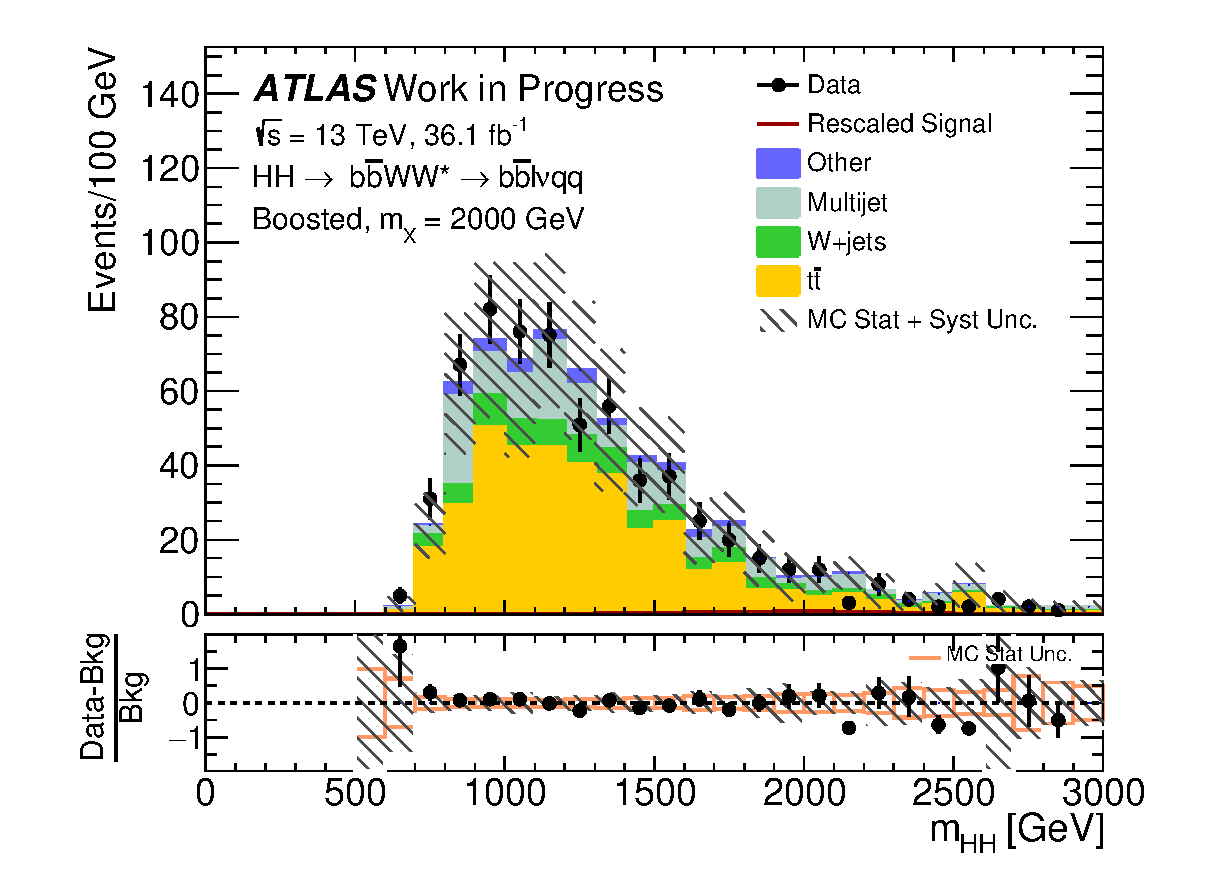
\includegraphics[width=0.5\textwidth]{figures/C_2tag_mbbcr_lepton_presel_met50_hhMassRebin1}
\end{center}
\end{frame}

\begin{frame}
\begin{center}
\header{Results}
\end{center}
\vspace{-0.2cm}
\begin{center}
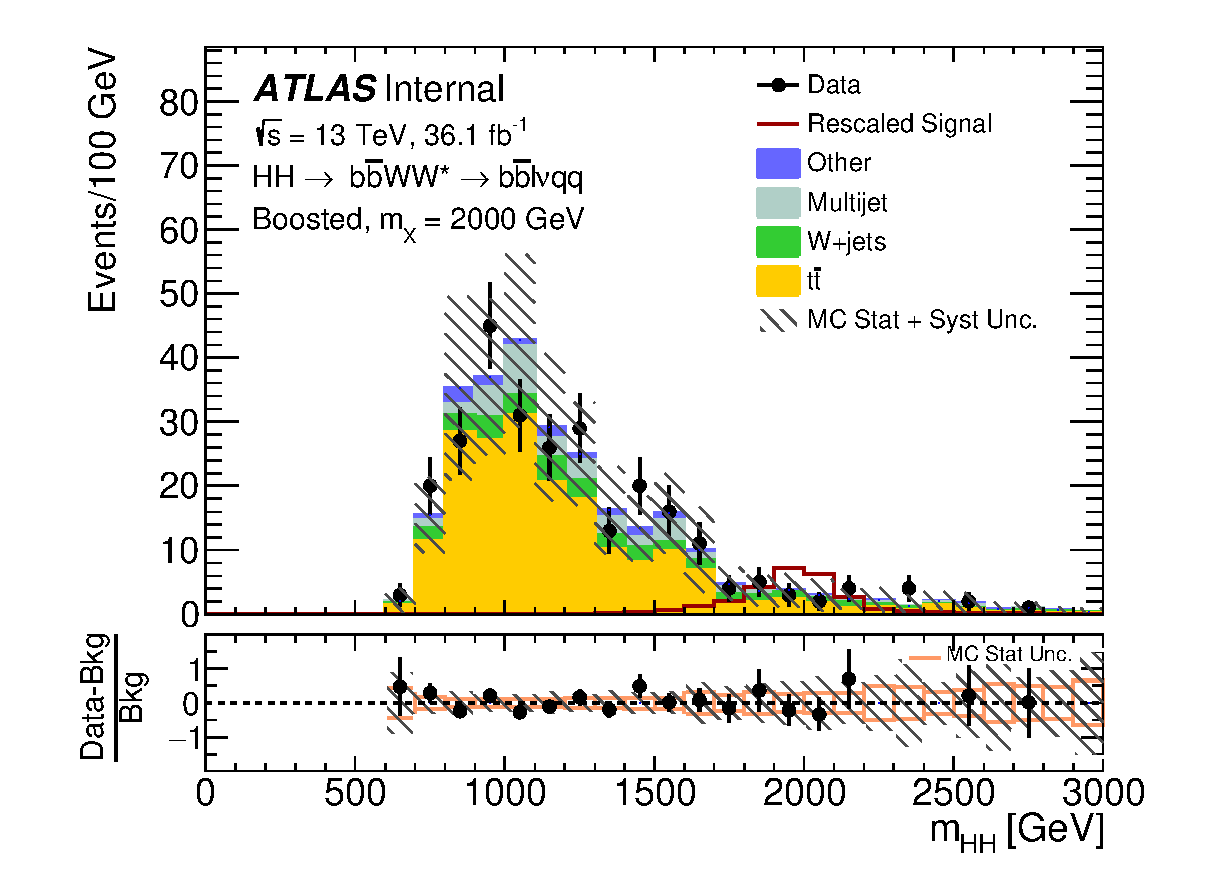
\includegraphics[width=0.9\textwidth]{figures/C_2tag_SR_lepton_presel_met50_hhMassRebin1}
\end{center}
\end{frame}

\begin{frame}
\begin{center}
\header{Results}
\end{center}
\begin{columns}
\begin{column}{0.5\textwidth}
\begin{center}
\color{MyPurple}{Published Analysis}
\includegraphics[width=01\textwidth]{figures/limit_2016_reOpt_HiggsApproved_Scalar_Paper_Combined_20190312_01}
\end{center}
\end{column}
\begin{column}{0.5\textwidth}
\begin{center}
\color{MyPurple}{Improved Analysis}
\includegraphics[width=01\textwidth]{figures/Final_limits}
\end{center}
\end{column}
\end{columns}
\end{frame}

\begin{frame}
\begin{center}
\header{Conclusion}
\end{center}
\begin{itemize}
\item Set the first limits for $HH$ resonant production over 1 TeV
\item Developed analysis for SM $HH$ production in $b\bar{b}l\nu$ channel
\begin{itemize}
\item Set limit of 300 X SM cross section
\end{itemize}
\item Improved the cross section upper limit for high resonant mass by $\sim$factor of 2
\end{itemize}
\end{frame}

\begin{frame}
\begin{center}
\header{Outlook}
\end{center}
\begin{itemize}
\item Move to Fatjet trigger
\begin{itemize}
\item Lepton ID requirement in derivation limits the high mass analysis
\end{itemize}
\item Neutrino reconstruction needs improved at high mass
\begin{itemize}
\item Use $H\rightarrow{}b\bar{b}$ information
\end{itemize}
\item ABCD estimate is limited by statistics
\begin{itemize}
\item Move to alternate QCD estimate like MM
\end{itemize}
\end{itemize}
\end{frame}

\begin{frame}
\begin{center}
Thank you to my committee:\\
Eric Torrence (Advisor)\\
Stephanie Majewski (Chair)\\
Tim Cohen\\
Hank Childs\\
And a special thanks to Alison
\end{center}
\end{frame}


\appendix
\backupbegin
\begin{frame}
\begin{center}
\fontsize{16}{8}\selectfont \textbf{{\color{MyPurple}{Backup}}}\\~\\
\end{center}
\end{frame}


\backupend
\end{document}


